\input{../../preamBeamer.tex} 
\input{../../variables.tex}

% Thèmes choisi : 

%\usetheme{Marburg} % Menu à droite
%\usetheme{Boadilla} % Sans menu bleu
\usetheme{CambridgeUS}  %Sans menu rouge^{}

\newcommand{\Nocours}{2}



% Debut - Rédaction du diaporama


\begin{document}
	
	
	\title[Les OS et Linux]{
		Cours \Nocours :\\ Installation système d'exploitation Linux}
	\author[\initiales]{\prof \\ DFC - Cégep de Sainte-Foy}
	\institute[\nomcoursCourt]{\nomcours\\ \cours 
	\vspace{2.5cm}
	\\ {\tiny Version du cours : \versionCours}}
	
	\date{\null}
	
	
	
	
	
	\begin{frame}
		\titlepage
	\end{frame}
	
	\begin{frame}
		
		\tableofcontents
		
	\end{frame}
	
	\section{Installation d’un système d’exploitation}
	% =================================================================================
	\begin{frame}[containsverbatim]
		\frametitle{Installation d’un système d’exploitation sur PC ou virtualité}
		\begin{itemize}
			\item  Pour installer un nouvel OS, il faut vérifier au préalable
			s'il y a besoin de mettre à jour le matériel du PC avant.
			\item Il faut aussi vérifier la pertinence, en matière de coût de
			mettre à jour le matériel versus acheter un nouveau PC.
			\item Matériel à vérifier :
			\begin{itemize}
				\item Carte mère, les interfaces de connexions, usb, rj45, vidéo, etc.
				\item CPU
				\item RAM
				\item Disque dur (taille et type) 
				\item Mémoire vidéo
			\end{itemize}
		\end{itemize}
	\end{frame}
	
	\begin{frame}[containsverbatim]
		\frametitle{Liste de compatibilité matérielle (HCL)}
		\begin{itemize}
			\item  La plupart des systèmes d’exploitation comportent
			une liste de compatibilité matérielle.
			\item Ces listes se trouvent sur le site Web du fabricant.
			\item Elles incluent la liste du matériel qui fonctionne avec
			le système d’exploitation.
		\end{itemize}
	\end{frame}
	\begin{frame}[containsverbatim]
		\frametitle{Raisons motivant une nouvelle installation :}
		\textbf{Sur PC :}
		\begin{itemize}
			\item Lorsqu’un ordinateur passe d’un employé à un autre
			\item Lorsque le système d’exploitation est corrompu
			\item Lorsqu’un nouveau disque dur de remplacement est installé sur un ordinateur.
		\end{itemize}
		\textbf{Virtualisé :}
		\begin{itemize}
			\item Développer des environnements de tests
			\item Développer des environnements de production
		\end{itemize} 
	\end{frame}
	
	\subsection{Procédures de configuration d’un disque dur}
	
	\begin{frame}[containsverbatim]
		\frametitle{Origine des fichiers :}
		\begin{itemize}
			\item  Installation d’un système d’exploitation sur un réseau à partir
			d’un serveur
			\item Installation à partir d’une copie des fichiers du système
			d’exploitation stockés sur le disque dur
			\item \textbf{Installation à partir des fichiers du système d’exploitation
			stockés sur un CD ou un DVD ou un ISO}
		\end{itemize}
	\end{frame}
	\begin{frame}[containsverbatim]
		\frametitle{Destination des fichiers :}
		\textbf{Partition et formatage}\\
		Le disque dur doit être divisé logiquement (partitionné) :\\
		\vspace{10pt}
		{\color{blue}Sur Windows : }\\
		\begin{figure}[!h]
			\centering
			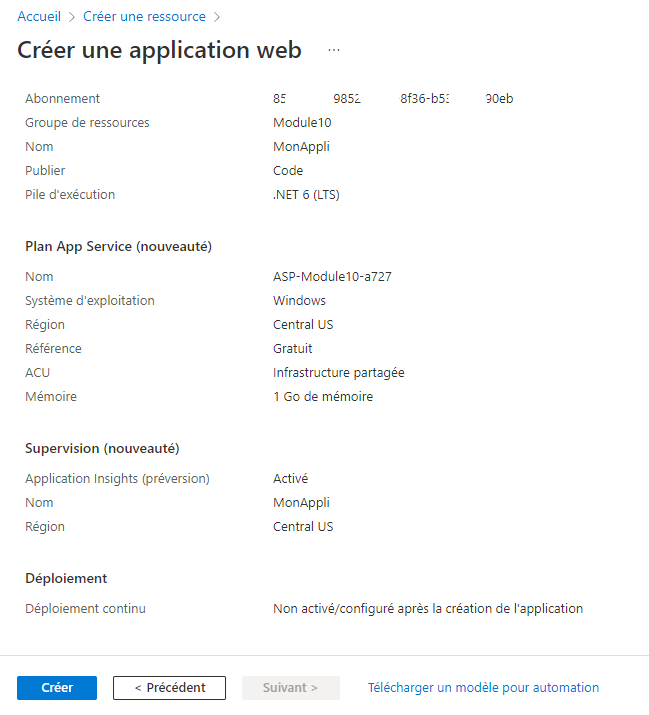
\includegraphics[scale=0.4]{images/capture1}
		\end{figure}
		
		{\color{blue}Sur Linux : }\\
		\begin{figure}[!h]
			\centering
			\includegraphics[scale=0.4]{images/capture2}
		\end{figure}
	\end{frame}
	\begin{frame}[containsverbatim]
		\frametitle{Pourquoi partitionner ?}
		Principalement pour des raisons de sécurité:
		\begin{itemize}
			\item  Si une partition est corrompue, le reste du système peut être encore accessible. Il peut suffire de restaurer une sauvegarde de la partition corrompue pour régler le problème. Mais aussi pour séparer les partitions qui risqueraient d'être submergées de fichiers (par exemple /var pour un serveur de courriel qui serait attaqué par un envoi massif...),le reste du système serait alors toujours opérationnel.
			\item Séparer les autres partitions de la racine "/" permet, en cas de corruption d'une autre partition, de toujours pouvoir amorcer Linux pour réparer le système...
			
		\end{itemize}
	\end{frame}
	\begin{frame}[containsverbatim]
	
		\begin{figure}[!h]
			\includegraphics[scale=0.2]{images/capture3}
			\caption{Formatage traditionnel}
		\end{figure}
		\begin{figure}[!htb]
			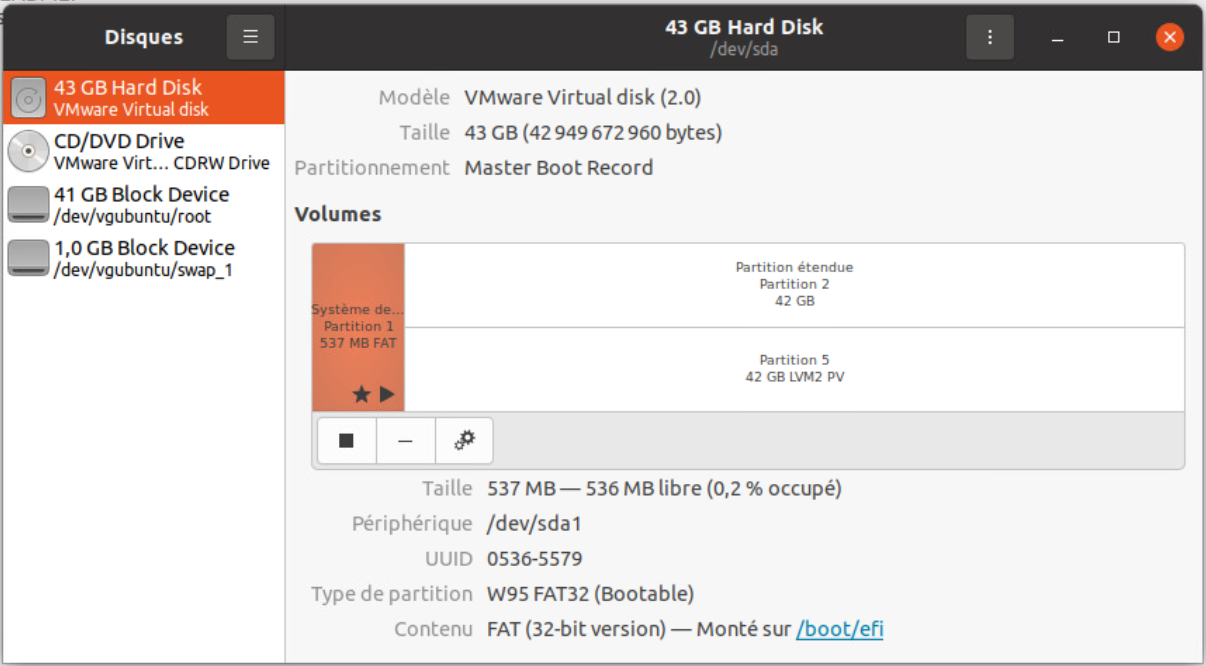
\includegraphics[scale=0.22]{images/Capture3b}
			\caption{Utillisation de LVM}
			\label{Fig1}
		\end{figure}
	\end{frame}
	\subsection{Procédure d'installation}
	\begin{frame}[containsverbatim]
		\frametitle{Procédure d'installation}
		Généralement les questions suivantes sont posées :
		\begin{itemize}
			\item  Langue
			\item Format de date, d’heure et de nombre (Fuseau horaire)
			\item Disposition du clavier (Canadien multilingue )
			\item Réseau DHCP ou fixe
			\item Type d’installation :
			\begin{itemize}
				\item  Standart formatage rapide peux de question
				\item Avancé : décider des partitions
			\end{itemize}
		\end{itemize}
	\end{frame}
	\begin{frame}
		\frametitle{IP fixe vs DHCP}
		\begin{figure}[!htb]
			\centering
			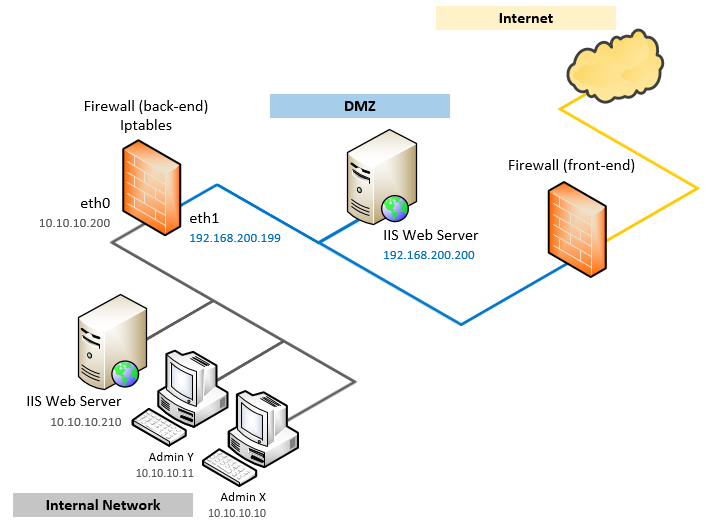
\includegraphics[scale=0.42]{images/dmz}
			\caption{DMZ versus réseau local}
			\label{Fig1}
		\end{figure}
	\end{frame}
	\section{Installation Ubuntu 20.04 LTS}
	\begin{frame}[containsverbatim]
		\frametitle{Installation Ubuntu 20.04 LTS}
		\textbf{Configuration minimale\footnote{Source : https://doc.ubuntu-fr.org/exigences\_minimales}}
		\begin{itemize}
			\item Version bureau :
			\begin{itemize}
				\item Processeur doubles cœurs de 2 GHz au moins
				\item 4 Go de RAM
				\item 25 Go d'espace de stockage.
				\item Une carte graphique affichant une résolution de 1024x768
				\item Média amovible :: Lecteur de DVD-ROM ou clé USB requis pour l'installation 
			\end{itemize}
			\item Version serveur : 
			\begin{itemize}
				\item Processeur de 1 GHz au moins
				\item 512 Go de RAM
				\item 1.75 Go d'espace de stockage.
				\item Média amovible : Lecteur de DVD-ROM ou clé USB requis pour l'installation  
			\end{itemize}
		\end{itemize}
	\end{frame}
	
	\subsection{Espace disque}
	
	\begin{frame}
		\frametitle{Noms attribués aux disques et aux partitions.}
		\begin{figure}[!h]
			\centering
			\includegraphics[scale=0.4]{images/capture6}
		\end{figure}
	Lecture complémentaire : \url{https://doc.ubuntu-fr.org/partitions}
	\end{frame}
	
	\subsection{Système de fichiers}
	\begin{frame}[containsverbatim]
		\frametitle{Système de fichier}
		L’action de « formater » un disque, une clé ou tout support de données consiste uniquement à créer sur un support de mémoire secondaire (volume de stockage) l’organisation logique permettant d’y placer des données. Le mot « formatage » sous Linux est utilisé pour décrire la création d’un système de fichiers. On parle donc de système de fichiers qui est à la fois l’organisation logique des supports au niveau le plus bas comme au niveau de l’utilisateur.
		
		Les informations ne sont pas écrites n’importe comment sur les disques. Une organisation est nécessaire pour y placer tant les informations sur les fichiers qui y sont stockés que les données. Ce sont le système de fichiers et les pilotes associés qui définissent cette organisation.\footnote{Rohaut, Sébastien 2020, Linux : {Préparation} à la certification {LPIC}-1 (examens {LPI} 101 et {LPI} 102) - [6e édition],}
	\end{frame}

	\begin{frame}[containsverbatim]
		\frametitle{Types de système de fichiers}
		Premiers systèmes de fichiers de Linux
		\begin{itemize}
			\item minix
			\item ext
			\item ext2 : standard sous Linux et reconnu par toutes les distributions
		\end{itemize}
		Systèmes de fichiers journalisés: 
		\begin{itemize}
			\item  \textbf{ext3} est une évolution de ext2 et a pour principale différence l'utilisation d'un fichier journal, lui permettant ainsi d'éviter la longue phase de récupération lors d'un arrêt brutal de la machine.
			\item \textbf{ext4} inclut un utilitaire de défragmentation natif travaillant au niveau des bits et gérant la défragmentation à chaud.
		\end{itemize}
	\end{frame}

\begin{frame}[containsverbatim]
	\frametitle{Types de système de fichiers}
	Les autres : 
	\begin{itemize}
		\item \textbf{XFS} : est le plus ancien des systèmes de fichiers journalisés sous Unix, datant de 1993. Est aujourd’hui la propriété de Red Hat qui en a fait son système de fichiers par défaut (RHEL, CentOS, Fedora). \\
		Outre ses capacités de stockage encore inimaginables aujourd’hui, il a un système de journalisation très performant et des mécanismes avancés comme la défragmentation en ligne la capacité de figer l’état du filesystem pour en effectuer un backup, le dimensionnement à chaud, la réservation de bande passante pour les entrées et sorties, une gestion avancée des quotas, et notamment sur des répertoires, etc.
		\item \textbf{VFAT} (Virtual File Allocation Table) est un terme générique regroupant les diverses versions de FAT supportant les noms de fichiers longs (255 caractères) sous Windows.
	\end{itemize}
\end{frame}
	
	\subsection {FHS}
	\begin{frame}
		\frametitle{Hiérarchie des systèmes de fichiers}
		\textbf{Filesystem Hierarchy Standard} (« norme de la hiérarchie des systèmes de fichiers », abrégé en \textbf{FHS}) définit l'arborescence et le contenu des principaux répertoires des systèmes de fichiers des systèmes d'exploitation GNU/Linux et de la plupart des systèmes Unix.\\
		
		La version actuelle est la 3.0 et fut publiée le 3 juin 2015\footnote{Source : https://fr.wikipedia.org/wiki/Filesystem\_Hierarchy\_Standard}. \\
		
		Ainsi, peu importe la distribution GNU/Linux (ou tout autre système d’exploitation adhérant à cette norme) que vous utilisez, vous serez en mesure de retrouver l’information que vous recherchez. 
	\end{frame}
	
	\begin{frame}
		\begin{figure}[!h]
			\centering
			\includegraphics[scale=0.4]{images/capture4}
		\end{figure}
		Source : \url{https://doc.ubuntu-fr.org/arborescence}
	\end{frame}
	
	\begin{frame}
		\begin{figure}[!h]
			\centering
			\includegraphics[scale=0.4]{images/capture5}
		\end{figure}
	\end{frame}

	\subsection{Partitions}
	\begin{frame}[containsverbatim]
		\frametitle{Les partitions  : root / }
		\begin{itemize}
			\item  \textbf{Point de montage :} / (obligatoire)
			\item \textbf{Utilité :} La partition racine est la base de l'arborescence de votre système Ubuntu. Par défaut, si aucun réglage n'est changé, c'est dans celle-ci que tous les fichiers vont être placés : fichiers de configuration, programmes, documents personnels, etc.
			\item\textbf{Taille :} Le minimum est 8 Go. Cependant, pour une question de confort, sa taille devrait être d'au moins 15 Go). Attention: si cette partition est pleine, votre Ubuntu ne pourra plus démarrer.
			\item \textbf{Type : }on choisira généralement EXT4 pour une installation sur disque dur
		\end{itemize}
	\end{frame}
	


\begin{frame}[containsverbatim]
	\frametitle{Partition swap (obligatoire)}
	\begin{itemize}
		\item  \textbf{Point de montage :} swap ( ne se voit pas à la racine)
		\item \textbf{Utilité :} L'espace d'échange (en anglais, swap space) est une extension de la mémoire vive (RAM) de votre ordinateur. Afin d'éviter un blocage de votre ordinateur lorsque sa RAM est pleine, Ubuntu se sert de cette partition pour décharger temporairement la RAM. Son utilisation à cet effet est plutôt rare dans les ordinateurs modernes, disposant d'au moins 1 Go de RAM. Cependant, elle sert aussi de décharge de la RAM lors de la mise en hibernation, c'est pour cette raison que la taille de la partition swap doit être d'au moins la taille de votre RAM si vous souhaitez utiliser cette fonction.
		\item\textbf{Taille :} Si vous avez moins de 1 Go de RAM, entre 1,5× et 2× la taille de votre RAM. Si vous avez plus de 1 Go de RAM, de 1× à 1,5× la taille de votre RAM. 
		\item \textbf{Type : } SWAP
	\end{itemize}
\end{frame}

\begin{frame}[containsverbatim]
	\frametitle{/home}
	\begin{itemize}
		\item  \textbf{Point de montage :} /home (fortement recommandé)
		\item \textbf{Utilité :} Lorsque vous disposez d'un disque dur suffisamment grand, un dossier home séparé permet d'isoler les paramètres personnels et les dossiers personnels des utilisateurs du reste du système.
		\item \textbf{Taille :} Selon votre usage.
		\item \textbf{Type : }on choisira généralement EXT4.
	\end{itemize}
\end{frame}

\begin{frame}[containsverbatim]
	\frametitle{/var}
	\begin{itemize}
		\item  \textbf{Point de montage :} /var 
		\item \textbf{Utilité :} contiens toutes les données variables (les messages électroniques, les sites web, le cache du système des paquets, les données de MySQL serveur, etc.). La place nécessaire dépend de l'usage que vous faites de votre ordinateur. La plupart du temps, la dimension de cette partition sera dictée par les outils de gestion des paquets qui prennent beaucoup de place.
		\item \textbf{Taille :} Pour une installation complète compter au moins 2 à 3 Go, une utilisation en serveur peut nécessiter plusieurs dizaines de Go.
		\item \textbf{Type : } on choisira généralement EXT4.
	\end{itemize}
\end{frame}


\begin{frame}[containsverbatim]
	\frametitle{/tmp}
	\begin{itemize}
		\item  \textbf{Point de montage :} /tmp
		\item \textbf{Utilité :} Partition pour les fichiers temporaires.
		Ceci est recommandé particulièrement pour les serveurs ou les ordinateurs dans lesquels il y a une modification fréquente de fichiers volumineux dont la taille peut augmenter drastiquement (comme en retouche photographique ou en montage de vidéos). Ce dossier contient les fichiers qui ne sont nécessaires que temporairement. Séparer le dossier des fichiers temporaires du reste de la partition racine garantit que les transactions en cours peuvent continuer même si la partition racine devient pleine ou, au contraire, que les transactions s'arrêteront par manque d'espace sans bloquer inopinément le système d'exploitation.
		\item \textbf{Taille :} Selon votre usage. De 2 à 4 Go est une suggestion.
		\item \textbf{Type : } on choisira généralement EXT4.
	\end{itemize}
\end{frame}
\subsection{Logical Volume Manager}
\begin{frame}
	\frametitle{Logical Volume Manager}
	Le gestionnaire de volumes logiques permet la création et la gestion de volumes logique sous Linux. L'utilisation de volumes logiques remplace en quelque sorte le partitionnement des disques.\\
	
	C'est un système beaucoup plus souple, qui permet par exemple de diminuer la taille d'un système de fichier pour pouvoir en agrandir un autre, sans se préoccuper de leur emplacement sur le disque.\\
	\vspace{10pt}
	\fcolorbox{black}{orange}{
		\begin{minipage}{11cm}
			\textbf{C'est essentiel dans la majorité des serveurs de données ou des serveur de bases de données sur site (on-premise).}
	\end{minipage}}
	
	
\end{frame}
\begin{frame}[containsverbatim]
	\frametitle{LVM }
	\begin{figure}[!h]
		\centering
		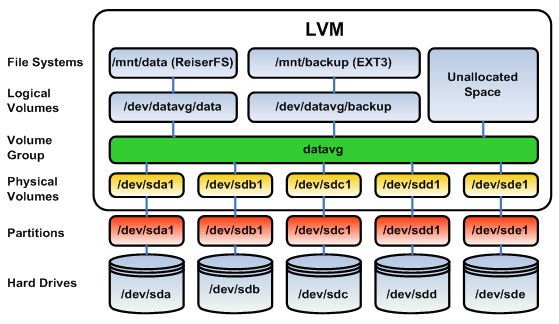
\includegraphics[scale=0.5]{images/Lvm1}
	\end{figure}
\end{frame}

% ======================================================
%\section*{Références}
%\begin{frame}
%	
%	\textbf{Références : } 
%	\bibliographystyle{apalike-fr}
%	\bibliography{../../biblio}
%
%	
%\end{frame} 
\section*{Droit d'auteur}

\begin{frame}[containsverbatim]
	\frametitle{Droit d'auteur}
	
	\textbf{Personne ayant contribué à la rédaction de ce document }
	\begin{itemize}
		\item  \href{mailto:jpduchesneau@csfoy.ca}{\Auteur}, \dateRedaction. Version : \versionDoc1
	\end{itemize}
	
	
	
	\vspace{1cm}
	
	\textbf{\textit{Ce document a été écrit avec LaTeX}.}\\
	
	\shadowbox{\parbox{11cm}
		{Cette oeuvre, création, site ou texte est sous licence Creative Commons Attribution - Pas d’Utilisation commerciale - Partage dans les Mêmes Conditions 4.0 International. Pour accéder à une copie de cette licence, merci de vous rendre à l'adresse suivante \url{http://creativecommons.org/licenses/by-nc-sa/4.0/} \\ ou envoyez un courrier à Creative Commons, 444 Castro Street, Suite 900, Mountain View, California, 94041, USA.}}
	
\end{frame}


\end{document}
% Fin - Rédaction du diaporama

